\section{Integration into Visualization Tools}

Throughout the lifespan of ECP, the VTK-m team operated in heavy collaboration with other ECP software technology teams.
The scope of the VTK-m portion of the project was to provide the fundamental technology to run scientific visualization algorithms on the GPU processors of the Exascale machines.
Other ECP teams, most notably the ALPINE project, developed tools that would leverage VTK-m while directly addressing application needs.
This arrangement avoided the redundant work of multiple teams developing their own visualization solutions and prevented users from having to use yet another software interface.
In this section we discuss the major visualization tools we integrated VTK-m with.

\ken{
  Each subsection should be roughly 1/2 page plus have an image demonstrating the tool with VTK-m that is about 1/3 page.
  (3 + 1/3 page total.)
  The subsection should start with a description of the tool.
  (Exception: the last subsection starts with a description of the lengthy process from committing code in VTK-m to it being available in a tool.)
  The following paragraphs describe how VTK-m is integrated at a high level.
  Avoid details like classnames.
}

\subsection{ParaView}

\assign{Sujin}

\subsection{VisIt}

\assign{Eric}

\subsection{Ascent}

\assign{Nicole}

\subsection{Alternate Delivery Mechanisms}

\assign{Tushar}
Integrating VTK-m filter into visualization software, e.g., ParaView, and VisIt, can be a lengthy process. For example, making a VTK-m filter available in ParaView requires going through multiple steps, including implemention of a VTK filter that wraps the VTK-m filter, continuous integration for VTK wrapper, and similar steps in ParaView. Such time-consuming software integration process can hinder the accessibility of VTK-m filters inside visualization tools, thus rendering VTK-m filters less effective in enhancing the pace of scientific discovery. 

Our ultimate goal is to make VTK-m filters practical for real use and to put tools in the hands of end users in a timely manner. One of the benefits that VTK-m offers is the easy exportation of VTK-m filters as plugins, which circumvents the tedious software integration process and makes VTK-m filters usable in ParaView and VisIt. For the plugin approach, the VTK-m filter still needs to be wrapped inside a VTK filter, but the time needed for the software integration and testing in VTK and ParaView can be bypassed.       

\begin{figure}[htb]
  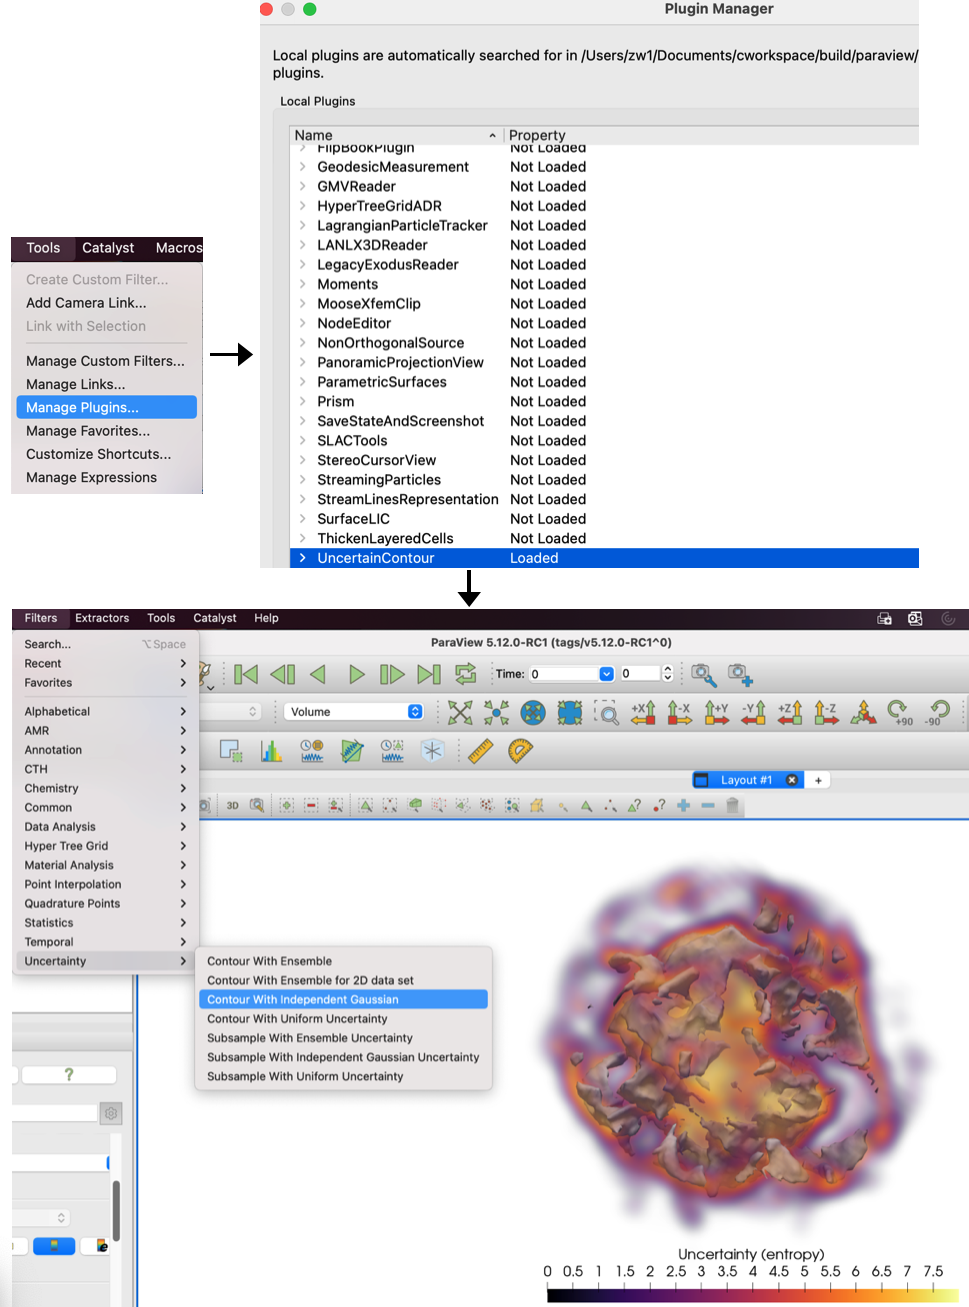
\includegraphics[width=\linewidth]{figures/isosurfaceUncertaintyPlugin.png}
  \caption{Integration of the VTK-m isosurface uncertainty filter into ParaView using the plugin approach for visualization of large-scale supernova simulations~\cite{Sandoval_2021}.}
  \label{fig:uncertainty-plugin}
\end{figure}

Figure~\ref{fig:uncertainty-plugin} illustrates the VTK-m isosurface uncertainty filter made available in ParaView using the plugin method. The isosurface uncertainty filter~\cite{wang2023funmc} is one of the major successes of the VTK-m library, as it is the first uncertainty visualization filter deployed for efficient large-data analysis. The filter enables interactive exploration of positional uncertainty in isosurfaces and overcomes difficulties related to the slowness of uncertainty computations. \tushar{Should we add here a link to the uncertainty filter in the master branch and add Nrushad as author?}. Using the plugin method depicted in Figure~\ref{fig:uncertainty-plugin}, VTK-m filters can be easily coupled with existing filters in ParaView for faster and better data understanding.

\ken{
  Talk about how you can deliver new functionality to these tools outside of the pipeline of implement in VTK-m $\rightarrow$ VTK $\rightarrow$ Tool.
  Use uncertainty plugin as an example of doing this.
}
